\documentclass{article}

% Tell me about my LaTeX bad practices
\usepackage[l2tabu, orthodox]{nag}
% For \hypersetup
\usepackage[pdftex]{hyperref}
% Gives us bigger margins on the right (and smaller on the left) for the margin
% paragraphs
\usepackage[left=2cm,
      top=2cm,
      right=2cm,
      bottom=1.5cm,
      marginparwidth=2cm,
      marginparsep=3mm]{geometry}
% For line brakes in tables
\usepackage{tabularx}
% For the split environment
\usepackage{amsmath}
% For scientific units
\usepackage{siunitx}
% For tabs in verbatim
\usepackage{moreverb}
% For fancy verbatim (use this one in mymulticol)
\usepackage{alltt}
% For wrapping figures in text
\usepackage{wrapfig}
% For a nice header
\usepackage{fancyhdr}
% For graphics
\usepackage{graphicx}
% For code listings
\usepackage{listings}
% For splitting long lists into columns
\usepackage{multicol}
% For no multicol on the kindle
\usepackage{environ}
\newif\ifmulticols
\NewEnviron{mymulticols}{
\ifmulticols
  \begin{multicols}{2}
    \BODY
  \end{multicols}
\else
  \BODY
\fi}
% Means you don't have to put \\ to start a new line.
\usepackage[parfill]{parskip}
% Make LaTeX pretty with better kerning etc
\usepackage{microtype}

\newcommand{\answer}[3]{
  \vspace{1em}
  \begin{minipage}[t]{0.85\textwidth}
    \textbf{#1}
  \end{minipage}
  \begin{minipage}[t]{0.15\textwidth}
    \begin{flushright}
      #3\\
      (#2 marks)
    \end{flushright}
  \end{minipage}
}

\pagestyle{fancyplain}

\author{Todd Davies}
\title{COMP28112 Model Answers}
\date{\today}

\begin{document}

\rhead{COMP28112 Model Answers}
\lhead{\today}

\maketitle

\section*{2011 Paper}

\answer{Describe one key difference between client-server and peer-to-peer
applications.}{2}{2011.1.a}

P2p does not have a central point of coordination; all nodes are the same in
terms of functionality (though they may have different roles). A client server
architecture is dissimilar to this in the fact that the machines that make up
the network have different capabilities and responsibilities that cannot be
changed.

\answer{Explain briefly what failures are known as Byzantine failures and what
the Byzantine generals problem refers to.}{2}{2011.1.b}

Byzantine failures are ones where processes send failed messages since they are
malicious or faulty.

The Byzantine Generals problem refers to a situation where two generals  are
situated on the sides of a valley and want to attack a city in the valley. To
win the battle, they must attack at the same time, but they cannot coordinate
their attack with any guarantee of timing it properly since they can only send
messages through the city where the messengers may be killed or the contents of
the message changed.

\answer{Describe briefly the two-phase commit protocol.}{2}{2011.1.c}

When a client wants to commit, it sends a message to a server. The server then
asks every client whether they are ready for a commit. Each client replies with
a yes/no. If there is a no, then a \texttt{global\_abort} message is sent,
otherwise a \texttt{global\_commit} message is sent. Upon receiving a global
commit or abort message, each client does exactly that, which ensures that only
one operation is done for all clients.

\answer{Explain briefly why somebody would choose to use Cloud
Computing.}{2}{2011.1.d}

\begin{itemize}
\item You don’t have to buy and own hardware, you can just rent time from other
  people’s hardware to do computing.
\item Clouds are large and therefore provide capacity for horizontal scaling.
\item Clouds make it easier to have the computing resources to apply techniques
  such as load balancing, replication and parallelization. This can make it
  easier to cope with variable demand.
\end{itemize}

\answer{Why is it practically impossible to achieve strict consistency in a
distributed system?}{2}{2011.1.e}

It is practically impossible to achieve strict consistency in a distributed
system since latency is not zero, so you can never know exactly what is going on
in a remote system at any one time. Messages can get lost or mutated too, which
further complicates the sending and updating of state between systems.

\answer{Suppose the C function below is to be made available to remote processes
using RPC. What particular implementation problem does this highlight? Why
is the normal solution only partly satisfactory?}{2}{2011.1.f}

\begin{verbatim}
  void doIt (int *p, int *q) { (*p)++ ; (*q)-- ; return ; }
\end{verbatim}

You would have to serialise and deserialise the values of p and q to have this
function run over RPC, because it uses pointers as opposed to actual values. You
would also have to update the value of the pointers either as they are updated
during the RPC function’s execution or after the function has finished
executing.

\answer{Distinguish carefully between a name server and a directory
server.}{2}{2011.1.g}

A name server takes the name of a resource and resolves it into the address of
the resource (e.g. a URL). A directory server takes attributes about an object
(e.g. the amount of RAM of a server or the age and course studied of a student)
and returns information about objects that have the same attributes (think LDAP)

\answer{What is meant by the term causally ordered multicast?}{2}{2011.1.h}

Ummmmm? Maybe take a look here:
\url{http://www.cse.buffalo.edu/~stevko/courses/cse486/spring13/lectures/12-multicast2.pdf}

Looks like every process has a vector clock and when a message is received, the
process waits until it can preserve the causal ordering before accepting the
message. This means it waits until messages that had been previously sent to it
(according to the vector clock) arrive before accepting the new message. Until
then, the message is buffered.

\answer{What properties are provided by a secure channel? }{2}{2011.1.i}

A secure channel is one that third parties cannot eavesdrop on. They might be
able to see the data passing through, but it will be encrypted somehow so they
won’t be able to make sense of it.

\answer{The Andrew File System (AFS) uses callback promises. Explain what this
means.}{2}{2011.1.j}

Dunno? Google turns up not much...

I’m guessing that it is a mechanism where if you send a remote server a message,
it promises to reply back to you and will cause a callback to execute in your
code when it does.

\newpage

\answer{Explain briefly why some applications are not parallelisable. Describe
Amdahl’s law and explain what it can be used for.}{3}{2011.2.a}

Some applications are not parallelisable because they have operations that are
interdependent. For example, if we were building a machine to compute how long
it takes for the collatz conjecture to reach 1 given an input number, we could
not parallelise it since each stage of the conjuncture depends on the last.
Amdahl’s law dictates how much we can speed up the execution of a program given
how much of the program is parallelisable. The law is:

\[
  \frac{1}{\text{serial portion} + (\frac{1}{\text{num threads}} \times \text{parallel portion})}
\]

\answer{Explain briefly what the four properties commonly denoted by the acronym
ACID are when referring to transactions.}{3}{2011.2.b}

ACID stands for:
\begin{description}
  \item \textit{Atomic} - All or nothing principle; either the transaction is
  committed and its changes are applied, or no state is changed as a result of
  the transaction.

  \item \textit{Consistent} - Each transaction moves the system from one valid
  and consistent state to another.

  \item \textit{Isolated} - Each transaction executes independently from all
  other transactions (even if they may be happening concurrently). The effect of
  transactions in progress is hidden from all other transactions.

  \item \textit{Durable} - Once a transaction is committed, it stays committed
  even in the event of failure such as power loss etc
\end{description}

\answer{A service is replicated onto 3 computers.}{6}{2011.2.c}

\begin{itemize}
\item The first computer, A, has a mean time between failures of 2 days.
\item The second computer, B, has a mean time between failures of 3.5 days.
\item The third computer, C, has a mean time between failures of 12 days.
\end{itemize}

\textbf{When a failure occurs, it takes on average 12 hours to fix.}

\answer{What is the availability of the replicated service?}{2}{2011.2.c.i}

We need to find the chance that all the computers will fail at the same time.
It is easy to find the up-times for each individual computer:

\begin{description}
  \item A - $75\%$
  \item B - $85.7\%$
  \item C - $95.83\%$
\end{description}

The chance that these will all fail at the same time is:
$(1 - 0.75) * (1 - 0.875) * (1 - 0.9853) = 0.00046 = 0.046\%$
Therefore, the uptime is going to be $100 - 0.046 = 99.954\%$

\answer{What would the availability of the replicated service be if only
computers A and B were used?}{2}{2011.2.c.ii}

If only A and B were used, it would be:

$1 - ((1 - 0.75) * (1 - 0.875)) = 0.96875 = 96.88\%$

\answer{Describe how in the general case of n computers, each with a mean
time between failures $f_i$ and an average time to fix a failure $t_i$ you
would choose the two computers that provide the highest
availability.}{2}{2011.2.c.iii}

Rank the computers in ascending order of $t_x/f_x$, and take the top $n$
elements.

\answer{The following four processes access a shared variable x. Each process
accesses a different replica of the store used to hold this variable. Before any
process starts executing, the value of x is 0 in all the replicas.}{8}{2011.2.d}

\begin{center}
  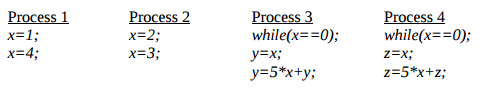
\includegraphics[width=0.5\textwidth]{images/2011-2-d}
\end{center}

\answer{When all four processes have completed executing the statements
given, are 7 and 14 possible values of y and z respectively, if the
replication uses the sequential consistency model? Justify your
answer.}{4}{2011.2.d.i}

With a sequential consistency model, it is not possible for the final values to
be $y=7$ and $z=14$, since for $y$ to equal $7$, $x$ must change state while
process $3$ is running, and this is not possible in a sequential consistency
model since only one process can execute at once.

The possible values of $x$ when process three actually starts are $x=4$ and
$x=3$, none of which let $y=7$.

\answer{When all four processes have completed executing the statements
given, are 7 and 14 possible values of y and z respectively, if the
replication uses the causal consistency model? Justify your
answer.}{4}{2011.2.d.ii}

Using a causal consistency model, we still can't get $y=7, z=14$, since we need
$y = 5 \times (x = 1) + (y = 2)$ and $z = 5 \times (x = 2) + (z = 4)$, but this
can never happen, since for $z = 4$, we need to have done $x = 1$, but  we need
to have done $y = 2$ before that, which means that we would have already done $x
= 2$.

\newpage

\answer{Describe in detail the Bully algorithm for the election of a leader in a
distributed system.}{8}{2011.3.a.i}

The Bully Algorithm works like this:

\begin{itemize}
\item An initiating client will send a message to all other clients with a
higher identifier than itself.
\item Any client receiving an election message will then start its own 
election, sending messages to clients with higher identifiers than itself.
\item Only when a process gets no replies (within a timeout) is it considered
elected. It then sends a message to all other processes announcing its election.
\end{itemize}

In this manner, any process that receives a message should always send a message
back to the sender

\answer{Carefully explain all the assumptions made in the Bully
algorithm.}{4}{2011.3.a.ii}

\begin{itemize}
  \item The timeouts are reasonable
  \item All processes know about all other processes (and their loads)
  \item Messages are delivered quickly
  \item Messages are delivered reliably
\end{itemize}

\answer{Describe one application for which the Bully algorithm might be applied,
indicating why a leader is needed.}{2}{2011.3.b}

In a peer-to-peer protocol (such as bit torrent), the Bully algorithm can be
used to elevate a node to coordinator status if the client that was coordinating
the network went offline or started to get a too high load.

\answer{In a system containing 6 computers, identified by the integers 1-6, the
leader is chosen by the Bully algorithm to be the live one with the highest
identifier. Assume for this part that all messages are delivered promptly, and
that the computers and the network are entirely reliable.}{6}{2011.3.c}

\answer{How many messages in total are sent so that the computer with
identifier 1 after it is rebooted can learn the identity of the leader by
triggering an election? Take care to explain your working!}{6}{2011.3.c.i}

Since identifier 1 is the lowest node, it will exhibit worst case behaviour for
the bully algorithm, $O(n^2)$.

This is because 1 will send five messages out (to each other process) to start
the election. Client 2 will then send out four messages (to the ones bigger than
it) etc, until there are $5 + 4 + 3 + 2 + 1 + 0 = 15$ messages sent. Since every
client receiving an election message replies to the sender, then $15$ replies
will be sent (in addition to the 15 initial message). Then, the winner of the
election (6) will send a message out to say that it is elected, which is another
$5$ messages, bringing the total to 35.

\answer{Repeat (i) with the computer rebooted and needing to discover the leader
being that with identifier 5 instead.}{2}{2011.3.c.ii}

If 6 wasn't online anymore, then the number of messages sent would be $(5 + 4 +
3 + 2 + 1) + (4 + 3 + 2 + 1) + 4 = 29$,


\newpage

\section*{2012 Paper}

\answer{What is a Java servlet?}{2}{2012.1.a}

A Java Servlet is a Java program with the capabilities of a server. It could
host web pages, provide an API endpoint or other services and is most commonly
used to serve content via the \texttt{HTTP} protocol.

\answer{What is the main assumption on which Cristian’s clock synchronisation
algorithm is based?}{2}{2012.1.b}

The time for a message to go from machine A to machine B is (roughly) the same
as the time it would take for a message to go from machine B to machine A. This
is most often accurate for routes with small round trip times.

\answer{Explain the difference between a name server and a directory
server.}{2}{2012.1.c}

A name server takes a name, matches it to an object and returns attributes about
the object. A directory server takes attributes, matches them to an object and
returns more attributes about the object.

\answer{Explain briefly what is meant by the term middleware.}{2}{2012.1.d}

Middleware is software that sits between a client application and the operating
system. It provides services to the client application that the operating system
does not, such as RPC stubs.

It can also provide an abstraction from the OS to mask the heterogeneity of
platforms used in distributed systems (some apps will run on Windows, others on
Linux, some on x64, some on ARM architectures etc).

\answer{Why is it practically impossible to achieve strict consistency in a
distributed  system?}{2}{2012.1.e}

Strict consistency is when any read to a shared data item returns the most
recent write operation on that data item. This means there must be an absolute
time ordering of all accesses. Unfortunately, since (as we know from the eight
fallacies of Distributed Computing), the latency of any network is not zero and
messages are not reliable. This means that any message we send to update other
machines about a change of state may not be sent. Since there is no way of
getting an absolute global clock or getting any global state, then we cannot
achieve real time memory consistency across all nodes, and therefore cannot
achieve strict consistency in the system.

\answer{Traditional RPC mechanisms cannot handle pointers. What is the
problem?}{2}{2012.1.f}

In order to handle pointers with RPC, you must serialise the datastructure into
a message so that it can be constructed from the same message at the other
machine. When the reply is received back at the sender, it can be deserialised
again and the values in the datastructure that were changed on the remote
machine can be updated in local memory. Traditional RPC mechanisms didn't have
this facility.


\newpage

\section*{2013 Paper}

\answer{Explain briefly what is meant by the term middleware.}{2}{2013.1.a}

Software that sits in between client applications and the operating system that
abstracts the details of implementing programming tasks and masks the
heterogeneity of the underlying platforms from the client application.

\answer{Explain briefly what failures are known as Byzantine
failures.}{2}{2013.1.b}

When a remote system either:

\begin{itemize}
  \item Does not reply to messages
  \item Sends faulty replies to message with miscellaneous data
  \item Sends maliciously crafted messages
  \item Acts inconsistently when interacting with different components
\end{itemize}

\answer{Describe briefly the two-phase commit protocol.}{2}{2013.1.c}

When a client wants to commit, it sends a message to a server. The server then
asks every client whether they are ready for a commit. Each client replies with
a yes/no. If there is a no, then a \texttt{global\_abort} message is sent,
otherwise a \texttt{global\_commit} message is sent. Upon receiving a global
commit or abort message, each client does exactly that, which ensures that only
one operation is done for all clients.

\answer{What is meant when a service is provided with at least once
semantics?}{2}{2013.1.d}

The application may send the RPC call multiple times before it receives word
from the server that the RPC call has taken place and was successful. This may
result in the RPC call being executed multiple times.

\answer{Why is it practically impossible to achieve exact synchronisation of
clocks in a distributed system?}{2}{2013.1.d}

The latency in a network is variable, so you can never know exactly how long a
message took to reach a server. Because of this, if one server sends its current
clock to another server, the latter one won't know how long it took for the
message to reach it and therefore it won't know how much to increment the clock
by.

Methods such as Cristian's algorithm and the Berkeley algorithm attempt to solve
this problem, but can only do so with some assumptions and to a limited
accuracy.

\answer{When using Java RMI, what is the purpose of the RMI
registry?}{2}{2013.1.f}

To act as a centeral repository for computers to access remote objects. Clients
can interrogate the registry using a string and get an object back. This allows
RMI methods to have parameters that are strings that point to objects in the
repository so you can pass arbitrary data structures and objects easily.

\answer{What is meant by parameter marshalling?}{2}{2013.1.g}

When an RPC call is made, the parameters cannot be sent directly (since they may
be pointers etc), so they must be serialized into a blob of text or binary data
before they are sent (marshalled) and deserialised at the other end by the
server (unmarshalled).

\answer{What is the key difference between caching and
replication?}{2}{2013.1.h}

Replication is keeping two fully fledged entities up to date with each other in
order to provide redundancy or distribute the load of a service over more
machines.

Caching is merely a small piece of hardware or a small program that remembers
the results of expensive computations after they've been done once and returns
the result without doing any computation if the same request comes again. Rarely
is there any business logic in a cache.

\answer{Explain briefly what Little’s Law is.}{2}{2013.1.i}

Little's law dictates that the average number of elements in a queue is:

\[
  \text{av. number} = \text{av. time between arrivals} \times \text{time to process one}
\]

This allows us to estimate how a system will handle load and what its queue size
will be (and if its appropriate).

\answer{In the context of lab exercise 2, what would you do to launch a denial
of service attack against the server?}{2}{2013.1.j}

\newpage

\section*{2014 Paper}

\answer{Explain briefly why the lack of homogeneity is a challenge when
developing distributed systems.}{2}{2014.1.a}

Since most of the individual computers that make up distributed systems will
differ, we need to come up with ways for them to communicate in such a way that
they can have meaningful interactions. This involves creating Interface
Definition Languages, middleware etc to help them inter-operate even when they
might be running different architectures.

\answer{Explain briefly why the assumption “latency is zero” is considered a
common fallacy in distributed computing.}{2}{2014.1.b}

Many (new) programmers haven't created applications intended to use distributed
systems before, and thus don't realise that waiting for a remote resource, RPC
call etc can (will) take orders of magnitude more time than a load from memory
might since it must travel through (many) different systems over different
protocols and even through different countries, where at any stage it may be
delayed and thus the latency increased.

\answer{Explain briefly what publish-subscribe messaging is.}{2}{2014.1.c}

Public-Subscribe messaging is when a `pub-sub' server is designated to take
messages from publishers and forward them to subscribers. The server provides a
central point at which systems can push their messages to and receive their
messages from and know that the message will be sent to/from the correct places.

This is especially handy if one client wishes to push a message to many (or
unknown amounts of) other clients. Instead of having to send $n$ messages, it
can send one message to the pub-sub server and the server will send out the
correct amount of messages to the subscribed clients. This helps abstract the
network topology away from clients.

\answer{In a distributed system, what is the purpose of an IDL?}{2}{2014.1.d}

An Interface Description Language defines an interface with which different
systems who may be running different architectures and different operating
systems etc can serialise data to and from and communicate safely.

They are commonly used by RPC software to facilitate the actual message sending
of the RPC calls.

\answer{In the context of RPC, what is copy-restore and what is it used
for?}{2}{2012.1.e}

Since a local client and a remote server (almost certainly) do not share memory
space, copy-restore is a way of letting one mutate the memory of another
remotely. On making an RPC call, the parameters for the method are serialised
and sent to the receiver, where they are deserialised again. While the procedure
is running, the parameters may be changed, and when the RPC call has finished,
they are serialised and sent back to the original machine, where their new
values are written back to memory.

\answer{What must a server do to provide at most once semantics to its
clients?}{2}{2014.1.f}

It must provide an acknowledgement to clients when it has received an RPC call
and successfully unmarshalled the parameters. This means that clients can know
not to re-sent the RPC call (since otherwise they wouldn't know that it was
received).

See \url{http://stackoverflow.com/questions/13330067/rpc-semantics-what-exactly-is-the-purpose}
for (what looks like) good description of at most once and at least once
semantics.

\answer{Explain briefly what failures are known as Byzantine
failures.}{2}{2014.1.g}

When a remote system either:

\begin{itemize}
  \item Does not reply to messages
  \item Sends faulty replies to message with miscellaneous data
  \item Sends maliciously crafted messages
\end{itemize}

Then it counts as a Byzantine failure.

\answer{In the context of data replication, explain briefly what eventual
consistency is.}{2}{2014.1.h}

When a protocol guarantees that data will eventually be consistent across
multiple systems, but it does not specify a time duration before the data will
be consistent (where consistency means to have the same data values).

\answer{When using Java RMI, what is the purpose of the
rmiregistry?}{2}{2014.1.i}

As a map between a String name of an object and the object's value. Clients can
query the rmiregistry with the name of an object and get the object back. In
this way, it acts as a distributed memory space for distributed systems, since
all systems can read and update the values stored in it.

The rmiregistry means that you aren't limited to just passing values in RPC
calls, you can pass references to objects and datastructures in the rmiregistry
and the system you're calling with the RPC call can look them up in the
rmiregistry.

\answer{In the context of lab exercise 2, what would you do to launch a denial
of service attack against the server?}{2}{2014.1.j}

Find the most expensive operation I can on the server (maybe listing the free
slots), and set up a program on a machine with a fast processor and high
bandwidth to run in a loop sending a request to the server every time it loops.
Thousands or tens of thousands of requests per second could be sent in the right
conditions, which could overload the server, cause it to cease responding (or at
least increase its response times) and deny its service to other users.

\answer{Explain briefly what the role of a client stub and a server stub is in
RPC.}{2}{2014.2.a}

Client stub:

\begin{enumerate}
  \item The client stub receives a request from the client application to
    execute an RPC call.
  \item It marshalls the parameters of the call into a binary or text blob and
    sends it (often in a format specified by an IDL) to the server.
  \item The client waits for a reply.
  \item When a reply is received, the client unmarshalls the parameters and
    updates them in the main memory.
\end{enumerate}

Server stub:

\begin{enumerate}
  \item When the server receives an RPC call from a client, it calls the server
    stub.
  \item The stub unmarshalls the parameters of the call and calls the local
    procedure with them.
  \item Once the procedure is finished, the parameters are marshalled back again
    and sent back to the client.
\end{enumerate}

\answer{Explain briefly what is meant by logical (Lamport) clocks and vector
clocks. What property is captured by vector clocks that is not if Lamport clocks
are used?}{3}{2014.2.b}

Logical and vector clocks aim to provide a happens-before ordering of events in
distributed systems. A logical clock is incremented every time an event occurs
in a distributed system, and it attached to all messages. If a client receives a
message with a higher logical clock than it, then its clock is updated to be
that value, and then it is incremented to signify that an event occurred (a
message received event).

A vector clock is like a logical clock, except each system keeps track of the
clock of each other system in a vector. In this manner, causality is captured by
vector clocks and not by logical clocks.

\answer{Explain briefly what the four properties commonly denoted by the acronym
ACID are when referring to transactions.}{4}{2014.2.c}

\begin{description}
  \item \textit{Atomicity} - Each operation/transaction must either succeed or 
  fail; there is no in-between. If the operation fails, then the state of the
  system must be exactly as it was before the start of the operation.
  \item \textit{Consistency} - Each operation or transaction must bring the
  state of the system from one valid state to another.
  \item \textit{Isolation} - Operations or transactions happening in parallel
  must execute as though they were running in a serial manner.
  \item \textit{Durability} - Once a transaction is committed or an operation
  is completed, the system will not roll back to a previous state in the event
  of failure or power loss etc.
\end{description}

\answer{Describe in detail how a centralised coordinating process can provide a
mutual exclusive access service in a distributed system.}{3}{2014.2.d.i}

A coordinating process acts as a lock server. If a process wants to enter a
section designated to be executed only in a mutually exclusive manner, then it
must first obtain a lock. It does this by asking the lock server for a lock,
executing the mutually exclusive section when it gets it, and releasing the lock
again once its done. If there is already a process in the mutually exclusive
section when another process asks for a lock, the lock server will put the
latter process in a queue until the first has finished with the lock.

\answer{When the machine supporting such a process gets overloaded with
other tasks it needs to find the least loaded machine in the network, and
pass over the provision of the mutual exclusive access service to a
process on that machine. Two algorithms are being considered for this.
The first is to have the server ask each machine about its workload and
then notify all the clients with the identity of the new server. The
second is to use a ring-based election, initiated by the current
server.}{8}{2012.2.d.ii}

\textbf{Fully describe the latter, clearly stating any assumptions you make and
compare it with the former with respect to the number of messages passed.}

A ring based election proceeds as follows:

\begin{enumerate}
  \item The initiator of the election will send a message to the next node
    containing its identifier (a pair of the name of the server and the
    reciprocal of its load).
  \item Each node will then forward the message if its identifier (the load) is
    lower than that of the message, or send its own identifier if its higher.
  \item The message goes around the circle until one node receives its own
    identifier.
  \item This means that the message has gone once around the ring and no other
    machine is more eligible for the role of coordinator, so the receiving
    machine considers itself elected.
  \item The newly elected coordinator then sends a message around the ring 
    announcing its election.
\end{enumerate}

The assumptions are that messages are sent reliably, and that no processes
crash.

This takes $O(3n-1)$ messages in the worst case, whereas the more simpler one
takes $O(3(n-1)) = O(3n - 3)$ messages, which although two fewer messages are
sent, is potentially worse since it requires each server to know about all other
servers.

\answer{Describe clearly all the operations that take place during a Remote
Procedure Call (RPC).}{4}{2014.3.a}

First, the client application will call the client stub with the procedure it
wants to execute and the parameters that are needed to do so. The client stub
then marshalls the parameters into a blob which is then sent to the server. The
server receives the message and the server stub unmarshalls the blob back into
parameters, which are then passed to the procedure on the server and the
procedure is ran. When the procedure is finished the server stub marshalls the
(possibly mutated) parameters back into a blob and sends it back to the client,
where the client stub will then unmarshal the parameters, update their values
in main memory and return to the client application.

\answer{Two computers are used to provide a replicated service. Each computer
has a mean time between failures of 12 days; a failure takes on average 12 hours
to fix. What is the availability of the replicated service?}{3}{2014.3.b}

Probability of failure = $1 - \frac{12}{(12 * 24) + 12} = 0.96$.

The probability of both machines failing at the same time is $0.96^2 = 0.9216 =
92.16\%$.

\answer{Consider a client-server application, which consists of 100 services
provided by some server. Ten of these services must be executed strictly one
after the other, not in parallel with any other services. The remaining 90
services may be executed concurrently and in any order. Assume that each service
takes the same time to execute. What is the maximum speedup that can be obtained
for the application if multiple identical servers are used to provide the
required services?}{3}{2014.3.c}

If ten services have to be executed in a serial manner, and the last 90 can be
executed in parallel then the maximum speed up using a number of parallel
processors is (using Amdahl's law):

\[
  \text{speedup} = \frac{1}{0.1 + (\frac{1}{\infty} * 0.9)} = 10\times
\]

\answer{Consider a simple server that carries out client requests without
accessing other servers. Explain why it is generally not possible to set a limit
on the time taken by such a server to respond to a client request. What would
need to be done to make the server able to execute requests within a bounded
time?}{4}{2014.3.d}

Since latency is variable, although we could try and ensure that the server
sends a response back to the client $n$ seconds after it has received a request,
we cannot make guarantees about how long it will take for the message to get
from the client to the server and back again.

Furthermore, we don't know how many requests the server might be dealing with, if
it has a queue of 1000000 requests, then it probably won't reply in the bounded
time.

The only way we might make such guarantees is by taking control of the network
and implementing some path through which packets can get from the client to the
server within a bounded time, and scaling the service horizontally so that more
server processes are online if the queue of requests starts to get large.

\answer{The following two processes access the shared variables x, y, z. Each
process accesses a different replica of the store used to hold these variables.
Before any process starts executing, the value of all three variables, x, y, z,
is 0 in all the replicas.}{6}{2014.3.e}

\begin{center}
  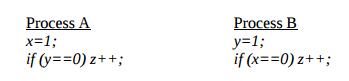
\includegraphics[width=0.4\textwidth]{images/2014-3-d}
\end{center}

\answer{When both processes have completed executing the statements given,
what are the possible values of z, if the replication uses the sequential
consistency model? Justify your answer.}{3}{2014.3.d.i}

If process A executes first, then the value of $z$ will be 1, and if process B
executes first then the value of $z$ will still be 1. This is because in both
cases, the \texttt{if} statement on the second process will fail.

\answer{When both processes have completed executing the statements given,
what are the possible values of z, if the replication uses the causal
consistency model? Justify your answer.}{3}{2014.3.d.ii}

The possible values are $z = {0,1}$ since if the statements $x=1;y=1;$ are
executed first, then both if statements will fail and $z=0$, if one process
fully executes before the other starts, then it will be the same case as in
\texttt{d.i}, and $z=1$, but $z$ can never be $2$ because either $x=1$ or $y=1$
before two of the if statements can be reached, so $z$ can never be incremented
twice.


\end{document}
